% Chapter 1

\chapter{Introduction} % Main chapter title

\label{Chapter1} % For referencing the chapter elsewhere, use \ref{Chapter1} 

\lhead{Chapter 1. \emph{Introduction}} % This is for the header on each page - perhaps a shortened title

%----------------------------------------------------------------------------------------
%\DeclareMathOperator*{\Min}{Min}
The goal in this thesis is to find a solution of the nonsmooth minimization problem

\begin{equation} \label{mainproblem}
  \begin{aligned}
    & \underset{x \in \mathbb{R}^n}{\text{min}}
    & & f(x) \\
    & \text{s.t.}
    & & l_i \leq x_i \leq u_i , \; \\
    & & & i = 1, \ldots, n.
  \end{aligned}
\end{equation}

where $f \colon \mathbb{R}^n \to \mathbb{R}$, $n$ is a very large but finite number. And $l_i$ and $u_i \in \mathbb{R}$

Larger problems not only mean that the problem will take a longer time to solve compared to a similar problem. But storing and calculating a Hessian matrix is prohibitively expensive. There a few techniques that have already been developed for the case when $n$ is very large and this is what we know as large scale optimization. Also, Several techniques have already been developed to handle this type of problems as long as the function $f$ is smooth. 

In this thesis $f(x)$ is a nonsmooth function.

For the particular case when $n$ is a small number, several methods that solve optimization problems of nondifferentiable functions in lower dimensions \citep{kiwiel85} have been developed. In the case of smooth functions, it is possible to use Newton iteration algorithms and achieve quadratic convergence, the problem with Newton algorithms is that they require second derivatives to be provided\footnote{the main issue with the second derivative is that it requires a total of $n \times n$ partial derivatives. Which is impractical for medium and for some small-size problems}. In the 1950's and several years after that, several quasi-newton methods were proposed where the second derivative Hessian matrix is "approximated" step by step \citep{unconstrained}. These approximations or "updates" are calculated after every iteration and the way in which this update is found defines a new method depending on the particular needs. This thesis will only be concerned with the $BFGS$. \footnote{BFGS stands for the last names of its authors Broyden, Fletcher, Goldfarb and Shanno} which can achieve super linear convergence, has proven to work in most practical purposes and posseses very nice self correcting features \citep{selfcorrecting}. In other words, it doesn't matter that one update incorrectly estimates the curvature in the objective function, $BFGS$ will always correct itself in just a few steps. This self-correcting property is very desired in the nonsmooth case, since changes in curvature could be large near the optimal point. $BFGS$ is not the right tool for large scale optimization and therefore an $L-BFGS$ adaptation is needed to solve the problem obtained on \ref{mainproblem}

A final assumption in this thesis is that the Hessian matrix is not sparse. In this case, there are other algorithms that may be more suitable \citep{Fletcher96computingsparse, sparse}, some of them have even been implemented in fortran \citep{lancelot}.

This thesis builds upon the original $L-BFGS-B$ code \citep{lbfgsbsoftware} that solves smooth problems of $f$. There were three main changes in the code. The first one is the line search conditions which required a small change in order to satisfy the different structure that a nonsmooth function requires. The second one is the line search methodology which was changed from a cubic interpolation to a bisection algorithm and last change in the thesis was the termination condition.

Nocedal's original algorithm consists of $2$ steps. In the first step most of the dimensions in the problem should be removed, making the problem a lot simpler. And in the second step there is some fine tuning to guarantee better than just linear speed of convergence.

\chapter{Original algorithm}
\label{ChapterConstraints} % For referencing the chapter elsewhere, use \ref{ChapterConstraints} 

The original algorithm \citep{mainpaper} has an accompanying software written on $FORTRAN$ \citep{lbfgsbsoftware} and this thesis builds upon that software by making sufficient changes to make it applied to the nonsmooth case.

\section{Gradient Projection}

The original algorithm was created for the case when $n$ is large and $f$ is nonsmooth. Its first step is a gradient projection similar to the one outlined in \citep{gradproj1, gradproj2} which is used to determine an active set corresponding to those variables that are bound at each step. The active set is defined at point $x^*$ is defined as:

\begin{equation}
  \begin{aligned}
    \mathcal{A}(x^*) = \{ i \in \{1 \ldots n\} |  x^*_i = l_i \vee  x^*_i = u_i\}
  \end{aligned}
\end{equation}

It seems like working on this active set is efficient in large problems and according to previous research \citep{nocedal} the gradient projection step is able to find most of the active set variables in a single stroke. 

In fact, A line search usually changes the active set by one variable at a time during the line search step \footnote{the line search is cut short immediately after the first bound is hit, so only one active constraint will change at every step. Unless the line search hits several constraints at the same time by coincidence, which is very unlikely}. So, if $1$ million constraints are active at a nondegenerate solution, at least $1$ million iterations will be needed just to get to that point.  Gradient projection gets rid of that problem, diminishing the number of iterations, and at the same reducing the number of variables for the next step.

Gradient projection works on the approximation model:

\begin{equation} \label{themodel}
  \begin{aligned}
    m_k(x) = f(x_k) + \nabla f(x_k)^T ( x - x_k) + \frac{(x - x_k)^T B_k (x - x_k) }{2}
  \end{aligned}
\end{equation}

Where $B_k$ will be a $L-BFGS-B$ approximation to the Hessian $\nabla^2 f$

In this first stage the algorithm starts on the current point $x_k$ searching on the direction of $-\nabla f(x_k)$. Whenever this search direction encounters one of the constraints, the search direction turns on the boundaries in order to remain feasible. The path is nothing but the feasible piecewise projection of the steepest descent search direction on the contraint "box" determined by the values $\overrightarrow{l}$ and $\overrightarrow{u}$. At the end of this stage, the value of $x$ that minimizes $m_k(x)$ on this piecewise gradient projection path is known as the "Cauchy point" $x^c$.

\subsection{Subspace Minimization}

The problem with gradient projection is that it eventually becomes steepest descent. In fact, gradient projection is exactly steepest descent if it were not for the existence of the constraints. The main problem with steepest descent is that it does not take advantage of the information of the curvature of the function which causes it to have a slow speed of convergence (linear). It is for this reason that a stage two is necessary. The idea is to use an $L-BFGS$ type of optimization only on the active set defined on the cauchy point $\mathcal{A}(x^c)$.

The idea at a higher level is to solve the constrained problem \ref{themodel}, but only on those dimensions that are free (not at bound). The starting point for this new problem will be the previously found cauchy point $x^c$, and the algorithm only moves in a direction that lives in the space of the free variables. In the end, the $L-BFGS$ approximation will provide a search direction $\hat{d}^u$

The algorithm will move in the direction set forth by $\hat{d}^* = \alpha^* \hat{d}^u$ where $\alpha^*$ is chosen so that the new point $\bar{x}_i$ satisfies some descent and curvature conditions, and stays within the constraints originally imposed. Once this step is finished the next step is deciding whether a new iteration is necessary or if the algorithm has finished.

\chapter{Modifications to the original algorithm}

\section{Convex Hull and termination conditions}

The most important requirement of a practical algorithm is that it ends in a finite time. For the case of smooth functions, the formal way to do this is to check whether the gradient has dimension zero $0$ wherever the constraints are not at bound. In the case of nonsmooth functions however, this is not necessarily true and the function at the minimum, may have a kink. In this kink the gradient may not vanish. Furthermore, if there is a sequence of points that approaches the optimum $x$ from the right, the gradients corresponding to this sequence of points might be completely different from the gradients associated to a sequence gradients associated to a sequence of points that approaches the optimum from the left. In other cases, the optimum might be located right at one of the boundaries, In this case the gradient does not necessarily vanish.

Given this set of conditions, there is the need for a special set of rules to establish the finalization of each optimization.

Since BFGS approximations typically converge to Clarke-Stationary points. The right methodology is to calculate the subgradient. One particular methodology that guarantees an end to the algorithm is suggested in \citep{overtonlewis}. In order to make sure that the gradient zero $\vec{0}$ is part of the subgradient calculated over a neighbourhood of the optimum.
The algorithm keeps a record of the latest gradient vectors in a small neighbourhood of the point that we suspect is the optimum, This collection is called $G_k$ in \citep{overtonlewis}, This collection of gradients spans an associated convex hull of gradients. If this convex hull contains at least one vector of dimension smaller than a tiny number $\tau_k$, the algorithm ends.

Of course the best way to find a vector with such properties is to find the vector with the minimal norm that resides in the convex hull generated by $G_k$

\subsubsection{minimization of the quadratic program}

This solution is guarantees to end up at a local optimum. However, one subalgorithm needs to be solved. This algorithm is a practical primal-dual algorithm. In this case in particular the best solution is to implement a variation of Mehrotra's Predictor-Corrector algorithm applied to quadratic programming. The primal dual method requires the solution of a system in order to calculate the search direction. The most expensive part of this solution is the calculation of the cholesky decomposition. Mehrotra's algorithm uses the same cholesky decomposition to calculate both directions. the predictor, and the corrector.

Currently there is not a theoretical calculation of the complexity of this algorithm but it is very used in practice. The implementation here is exactly the one on \citep{Nocedal}. It was implemented in fortran as part of the optimizer.

\section{cubic interpolation replaced with line search}

The original software by Nocedal\citep{Nocedal}, included a cubic line search. The idea of a cubic interpolation line search is to take advantage of the smooth properties of functions and take advantage of the curvature properties. It is debatable to see which one works better whether a simple line search or a cubic interpolation. However, In the case of nonsmooth functions, this line search does not serve our purpose and therefore a more typical line search that implements a bisection was used.

In general, a step length is selected. If this step length does not satisfy the sufficient decrease and curvature conditions, then a step length of half or double the size is selected. the algorithm is guaranteed to converge under a careful selection of the parameters, however, in case this does not happen, the software will stop with a warning. 

\section{the functions to be tested}

In order to make some tests, a few functions will be evaluated. The most important function to test this non-smooth optimizer is a modified version of rosenbrock's:

\begin{equation}
    f(x) = (x_1 - 1)^2 + \sum_{i = 2}^n |x_i - x_{i - 1}^2|^p
\end{equation}

Where the value of $p$ changes the behaviour of the optimizer. This function can be proven to be lipschitz continuous whenever $p > 1$ if restricted to the domain defined by 

\begin{equation}
  \begin{aligned}
    x_i = 
    \begin{cases}
      [-100, 100] & \text{if } i \in \text{ even numbers} \\
      [10, 100] & \text{if } i \in \text{ odd numbers}
    \end{cases}
  \end{aligned}
\end{equation}

and in fact, whenever the function is restricted to a finite domain. Because whenever $p > 1$ we have that the function $f(z) = |z|^p$ is zero $0$ around zero because the derivative $p |z| ^{p-1}$ is zero whenever $z$ tends to zero from the right. (from the left also because it is an even function). However the second derivative will not be as nice.

For the case when $p \leq 1$ we have that the second derivative tends to infinity. $\displaystyle \lim_{x \to 0^+} {f' = \infty}$. Which is already well known given the "heavyside" look of $f(z) = |z|$.

The convergence of the algorithm smoothly descends to the objective 
\centering
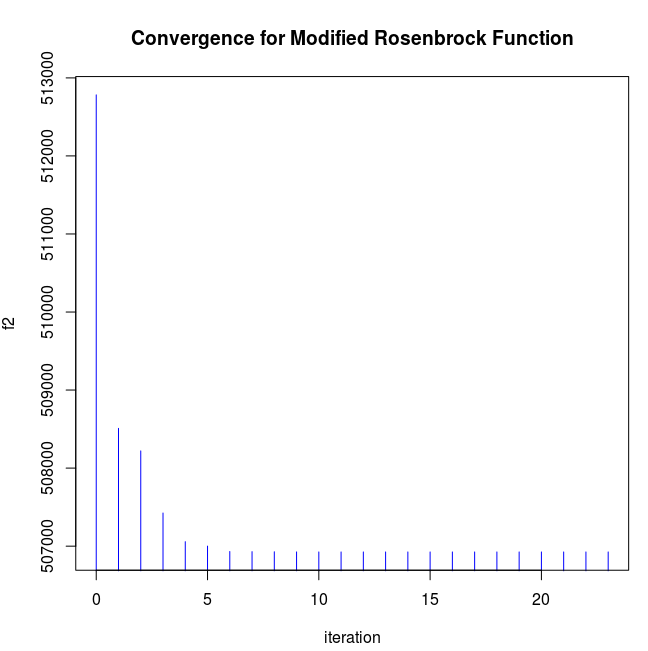
\includegraphics[scale=0.3]{Figures/convergence.png}

The converge is adversely affected by the selection of $p$ as one would expect. Values of $p$ descending to $1$ make the function less "smooth" and have the adverse effect of making the convergence much more difficult. In this exercise it is noticeable how slow the convergence becomes for a few specific values of $p$. In particular for $1.0001$

\centering
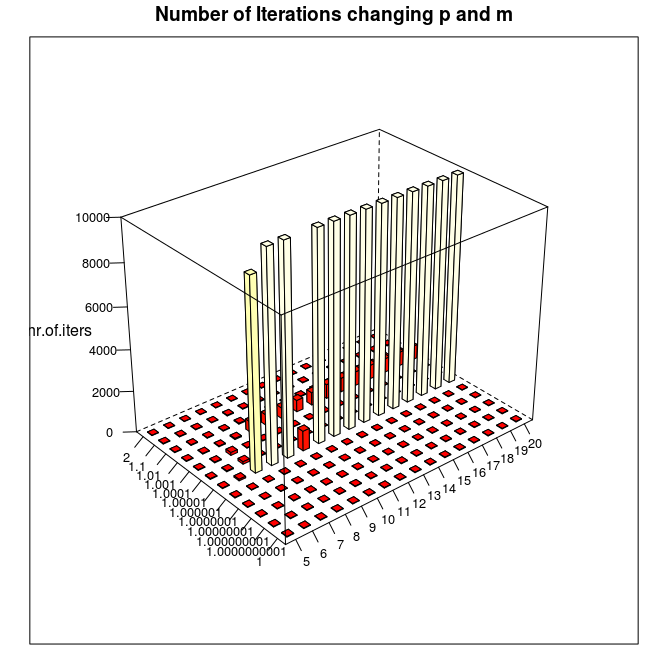
\includegraphics[scale=0.3]{Figures/hist3dmpniter.png}

\section{Weak wolfe conditions}

Probably the most important change made to the original code was the change in the curvature condition. Originally there are two Wolfe conditions, one of them is the Armijo condition, also known as the sufficient decrease conditions.

\begin{equation}
  \begin{aligned}
    f(x_k + \alpha_kp_k) \leq f(x_k) + c_1 \alpha _k p_k^T\nabla f(x_k)
  \end{aligned}
\end{equation}

and the other one is the curvature condition, of which the most popular version is the strong wolfe curvature condition:

\begin{equation}
  \begin{aligned}
    |p_k^T \nabla f(x_k + \alpha _k p_k)| \leq |p_k^T \nabla f(x_k)|
  \end{aligned}
\end{equation}

The strong wolfe is a more natural way to see and achieve convergence, but the problem is that it does not work well for the nonsmooth case. This is because near the minimal points, there maybe abrupt changes in curvature, in these cases there is no other option but to relax the curvature condition as long as the sufficient decrease condition is satisfied. The suggested new decrease condition is this.

\begin{equation}
  \begin{aligned}
    p_k^T \nabla f(x_k + \alpha _k p_k) \geq p_k^T \nabla f(x_k)
  \end{aligned}
\end{equation}

It is noticeable that with this new condition the algorithm does not crash, as opposed to when the hard wolfe condition is used.
